%
%                       This is a basic LeTeX Template
%                       for the First Year PhD literature review 
\documentclass[a4paper,12pt]{article}
\usepackage{head,fullpage}     % Add local fullpage and head macros
\usepackage[pdftex]{graphicx}  % Add graphicx pachage with pdf flag (must use pdflatex)
\usepackage{wrapfig, subcaption, setspace, booktabs}
\usepackage{datetime}
\usepackage{xcolor}
\definecolor{tcd-blue}{HTML}{0569b9}
\definecolor{tcd-lightblue}{HTML}{448fcb}
\usepackage[colorlinks=true,citecolor=tcd-blue,linkcolor=tcd-lightblue]{hyperref}
\usepackage{amsmath}
\usepackage{cleveref}
\usepackage[round]{natbib}
\bibliographystyle{abbrvnat}
\usepackage{float}
\usepackage{setspace}
\usepackage{imakeidx}
\usepackage{caption}
\usepackage{subcaption}
\makeindex

% Set 1.5 spacing
\onehalfspacing

% Custom Colours 


% --- Commands --- 
\newcommand{\smass}{\, \text{M}_\odot}

\newcounter{daggerfootnote}
\newcommand*{\daggerfootnote}[1]{%
    \setcounter{daggerfootnote}{\value{footnote}}%
    \renewcommand*{\thefootnote}{\fnsymbol{footnote}}%
    \footnote[2]{#1}%
    \setcounter{footnote}{\value{daggerfootnote}}%
    \renewcommand*{\thefootnote}{\arabic{footnote}}%
    }

\newdateformat{monthyeardate}{%
  \monthname[\THEMONTH], \THEYEAR}
\parindent=0pt          %  Switch off indent of paragraphs 
\parskip=5pt            %  Put 5pt between each paragraph  

\begin{document}
\begin{minipage}[b]{110mm}
        {\LARGE\bf School of Physics %\\and Astronomy
        \vspace*{17mm}}
\end{minipage}
\hfill
\begin{minipage}[t]{40mm}               
        \makebox[40mm]{
        
\includegraphics[width=40mm]{assets/tcd.logo.png}}
\end{minipage}
\par\noindent                                           % Centre Title, and name
\vspace*{2cm}
\begin{center}
        \Large\bf The Fast Transient Sky\\
        \normalsize \textit{Stage Transfer Report}
\end{center}
\vspace*{1.5cm}
\begin{center}
        Owen Johnson\daggerfootnote{ojohnson@tcd.ie}\\ 
        Astrophysics Group\\ 
        \monthyeardate\today            % Submission Date
\end{center}
\vspace*{5mm}
%
%                       Insert your abstract HERE
%                       
\begin{abstract}
        The abstract is a short concise outline of your 
        project area, {\bf of no more than 100 words}.
\end{abstract}

\vspace*{1cm}

% \vspace*{3cm}
% Signature:\hspace*{8cm}Date:

\vfill
{\bf Supervisor:} Assoc. Prof. Evan Keane          
\newpage
%                                               Through page and setup 
%                                               fancy headings
\setcounter{page}{1}                            % Set page number to 1
\footruleheight{1pt}
\headruleheight{1pt}
\lfoot{\small School of Physics}
\lhead{Stage Transfer Report}
\rhead{ \thepage}
\cfoot{}
\rfoot{Date: \today}
%
{
\hypersetup{linkcolor=black}
\tableofcontents 
} 
\thispagestyle{empty}         
\newpage 
                      % Makes Table of Contents

% \vspace*{\fill}
\section*{Declaration}
I hereby declare that this report is entirely my own work and that it has not been submitted as an exercise for a degree at this or any other university.

I have read and I understand the plagiarism provisions in the General Regulations of the University Calendar for the current year, found at \url{http://www.tcd.ie/calendar}.

\vspace{1cm}

Signed:~\rule{5cm}{0.3pt}\hfill Date:~\rule{5cm}{0.3pt}

\vspace*{\fill}
\newpage

\section*{Publications and Presentations}
\subsection*{Publications}

\textbf{Johnson, O.A}., Gajjar, V., Keane, E.F., et. al (2023). Simultaneous dual-site SETI with LOFAR international stations. Manuscript accepted for publication to AJ. arXiv:2310.15704

\subsection*{Presentations}
\begin{enumerate}
\item Low Frequency's Place in SETI, January, 2024, PSETI Symposium, Penn State. \hfill \textbf{[Invited]}
\item Technosignatures with NenuFAR, December, 2023, Science at Low Frequencies IX, UvA. 
\item SETI Science at 30 - 190 MHz, November, 2023, BLUK Workshop, SKAO.\\ \textbf{[Invited]}
\item Technosignature Science at Low Frequencies, November, 2023, NASA Goddard Flight Center. \hfill \\ \textbf{[Invited]}
\item Dual Site SETI Searches, 2023, International Astronautical Congress, Baku. 
\end{enumerate}

\newpage
\section*{Physical Constants}
\vspace*{\fill}
\begin{table}[H]
        \centering
        \begin{tabular}{|c|c|c|}
                \hline
                Constant & Symbol & Value \\
                \hline
                Speed of Light & $c$ & $2.99792458 \times 10^8 \text{ m/s}$ \\
                Gravitational Constant & $G$ & $6.674 \times 10^{-11} \text{ m}^3 \text{ kg}^{-1} \text{ s}^{-2}$ \\
                Planck's Constant & $h$ & $6.626 \times 10^{-34} \text{ m}^2 \text{ kg} \text{ s}^{-1}$ \\
                Boltzmann Constant & $k_B$ & $1.381 \times 10^{-23} \text{ m}^2 \text{ kg} \text{ s}^{-2} \text{ K}^{-1}$ \\
                Stefan-Boltzmann Constant & $\sigma$ & $5.670 \times 10^{-8} \text{ W} \text{ m}^{-2} \text{ K}^{-4}$ \\
                Electron Charge & $e$ & $1.602 \times 10^{-19} \text{ C}$ \\
                Electron Mass & $m_e$ & $9.109 \times 10^{-31} \text{ kg}$ \\
                Proton Mass & $m_p$ & $1.672 \times 10^{-27} \text{ kg}$ \\
                Neutron Mass & $m_n$ & $1.675 \times 10^{-27} \text{ kg}$ \\
                Solar Mass & $M_\odot$ & $1.989 \times 10^{30} \text{ kg}$ \\
                Solar Radius & $R_\odot$ & $6.957 \times 10^8 \text{ m}$ \\
                Solar Luminosity & $L_\odot$ & $3.828 \times 10^{26} \text{ W}$ \\
                Solar Temperature & $T_\odot$ & $5772 \text{ K}$ \\
                Jansky & Jy & $10^{-26} \text{ W} \text{ m}^{-2} \text{ Hz}^{-1}$ \\
                \hline
        \end{tabular}
\end{table}
\vspace*{\fill}

\newpage
\setcounter{page}{1} 
\section{A Prelude to Pulsars} \label{sec:prelude}
When stars with a mass of at least $8 \smass$ reach the end of their evolutionary stage they experience a depletion of nuclear fuel will and undergo a core collapse.  This results in the star exploding as a Supernova. Depending on the mass of the host star the Supernova will form a black Hole or a neutron Star. Based on the electron degeneracy pressure limit \citep[pp. 434 - 443]{chandrasekhar_introduction_2012} stars that fall in the range of 20 - 30 $\smass$ form neutron stars \citep{heger_how_2003}. \\

Neutron stars are supported against further collapse by the presence of neutron degeneracy pressure which arises from the Pauli exclusion principle. Strong Nuclear forces between the neutrons also provides additional support against gravatational collapse. With these two opposing forces a stable equilibrium is formed. \\ 

In turn, this makes neutron stars exceptionally dense, they are the densest known objects in the universe that emit light. The average density of a neutron star is $10^{17} \text{kg/m}^3$ \citep{baym_neutron_1971} and their radii are comparable to the size of cities, with radii of 10 - 20 km. \\

During collapse the conservation of magnetic flux plays a crucial role in the large strength magnetic fields that are observed in neutron stars along with contributions from the dynamo effect and frozen-in magnetic fields. The strength of a pulsar's magnetic field is on the order of $10^{12}$ - $10^{15}$ Gauss \citep{michel_theory_1982}. \\

Charged particles accelerate along the magnetic field lines in the magnetosphere of the neutron star. These particles emit electromagnetic radiation in a cone shape along the magnetic axis. If the magnetic axis is not aligned with the rotational axis of the neutron star, the radiation beam will sweep across the sky. This is known as a pulsar, a Galacic lighthouse.% analogus to cosmic lighthouses. 

\subsection{The Population of Pulsars}

At the time of writing there are currently more than 3380 known pulsars. Since their discovery by Jocelyn Bell Burnell \citep{hewish_observation_1968} the population has grown immensly but there remains many open questions about pulsar evolution and the subclasses that lie within the population as a whole. Similarly to how exoplanet popilations are shown using the mass-radius diagram and stellar populations are shown using the Hertzsprung-Russell diagram, pulsar populations are shown using what is known as the $P-\dot P$ diagram. \\

$P$ representing the Pulsar's rotational period and $\dot P$ it's derivative. These are key ways that pulsars are classified and study in context of their evolution. An example of a $P-\dot P$ diagram is shown in \cref{fig:p-pdot}. Different values on the plot indicate the roughly the Pulsars age and magnetic field strength. \Cref{fig:p-pdot} shows the vastly different values bettween pulsars in the milisecond range and pulsars in the second range. \\ 

Theoretically it has been shown that pulsars exhibit a death line in the $P-\dot P$ diagram. This is the line where pulsars are no longer able to emit radio waves. This is due to the pulsar's magnetic field is no longer strong enough to accelerate particles along the magnetic field lines. However it has been shown that pulsars do exist below this line. The area below this line is commonly referred to as the "graveyard". \\
\begin{figure}
    \centering
    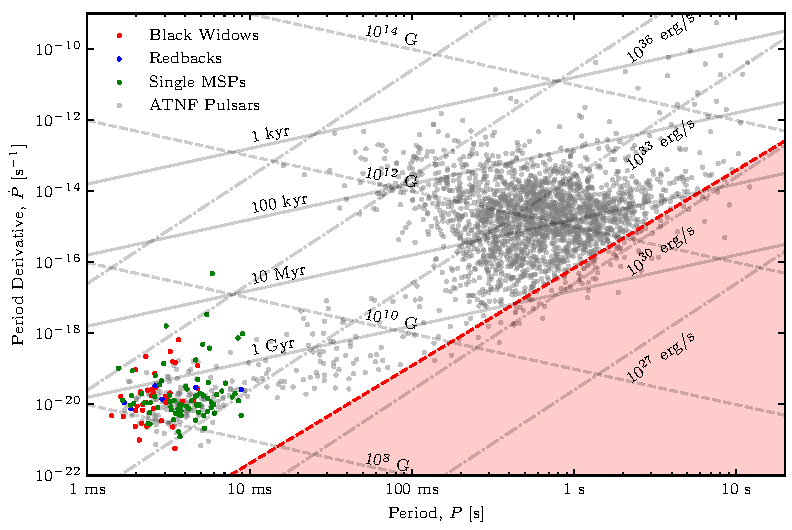
\includegraphics[width=0.8\textwidth]{figs/PPdot-diagram.pdf}
    \caption{The $P-\dot P$ diagram showing the population of pulsars. The the milisecond pulsar subclasses are colour coded. The red region represents the death line, where pulsars are theortically no longer able to emit radio waves.}
    \label{fig:p-pdot}
\end{figure}

\subsection{The Properities of Pulsars}

The following section gives a breif non-exhaustive overview of some of the key properities of pulsars. 

\subsubsection{Neutron Star Radius \& Mass}

Understanding the mass of pulsars are important for understanding their evolution and equation of state. \cite{oppenheimer_massive_1939} derived a canonical mass limit of neutron stars to be 1.4 $\smass$, but expermientally this has been shown to be higher with the largest mass of a pulsar being $\sim 2.35 \smass$ \citep{Romani_2022}. The mass-radius relationship of a pulsar is defined by an equation of state and a maximum mass limit. Redshifts and gravatational effects observed in pulsars exhbit the observed temperture and flux to be smaller than the actual value. The observed radius $R_\text{obs}$ can be described as follows \citep{pulsar_handbook}, 

\begin{equation}
    R_\text{obs} = \frac{R}{\sqrt{1 - \frac{2GM}{Rc^2}}} = \frac{1}{R} \sqrt{1 - \frac{R_s}{R}}
\end{equation}

where $R$ is the pulsar's radius and M is the gravatational mass, $G$ is the gravatational constant, $c$ is the speed of light and $R_s$ is the Schwarzschild radius. \\ 
The lower limit of the neutron star radius is decribed by 

\begin{equation}
    R_\text{min} \simeq 1.5 \ R_s = \frac{3GM}{c^2} = 6.2 \ \text{km} \left( \frac{M}{1.4 \smass} \right)
\end{equation}

Opposite to this upper limit of the radius is obtained by requiring that there is stability against breaking up due to centrifulgal forces. This gives \cref{eq:radius-max} following as described in \cite[p.~58]{pulsar_handbook}. 

\begin{equation}
    R_\text{max} \simeq \left(\frac{GMP^2}{4 \pi^2}\right)^{1/3} = 16.8 \ \text{km} \left( \frac{M}{1.4 \smass} \right)^{1/3} \left( \frac{P}{\text{ms}} \right)^{2/3}
    \label{eq:radius-max}
\end{equation}

Most pulsars are observed to have radii in the range of 10 - 15 km \citep{lattimer_neutron_2001}, giving them the unique position of 'almost' black holes. 

\subsubsection{Spin Evolution}
One of the most unique characterstics of pulsars is the spinning that they exhibit. Understanding the spin evolution gives insight into many parameters of the pulsars most notable the stage of their evolution. Pulsar's begin their life in the upper end of the $P-\dot P$ diagram and slowly move down and to the right as they age due to a loss in rotational energy, commonly referred to as spin-down luminosity. The spin-down $(\dot E)$ is decribed as follows  \citep[p.~59]{pulsar_handbook}, 

\begin{equation}
    \dot E  = - \dfrac{dE_{\text{rot}}}{dt} = 4\pi^2 I \dot P P^{-3}
    \label{eq:spin-down-energy}
\end{equation}

Where $I$ is the moment of inertia. It is important to note that the energy loss that is converted into radio emmision is almost negligable in comparison to the total energy loss from spin down. 

% \subsubsection{Radio Emission Beam}

% Pulse width

% \begin{equation}
%     \cos \rho = \cos \alpha \cos (\alpha + \beta) + \sin \alpha \sin (\alpha + \beta) \cos \left( \frac{W}{2} \right)
% \end{equation}

\subsubsection{Braking Index}

Pulsar's have strong magnetic dipoles, according to classic mechanics a rotating magnetic doplole that exhibts a moment, $|m|$ emits an electromagnetic wave at the pulsars rotation frequency \citep[p.~60]{pulsar_handbook}. The dipoles radiation power is characterized by, 

\begin{equation}
    \dot E_{\text{dipole}} = \frac{2}{3c^3} |m|^2 \omega^4 \sin^2 \alpha
\end{equation}

Where $\alpha$ is the angle between the magnetic axis and the rotation axis. Equating the above equation to the loss of rotational energy described in \cref{eq:spin-down-energy} gives the following for the expected evolution of the period, 

\begin{equation}
    \dot \Omega = - \frac{2}{3Ic^3} |m|^2 \Omega^3 \sin^2 \alpha
\end{equation}

This is more commonly written ass a power law, 

\begin{equation}
    \dot \nu = -K \nu^n 
    \label{eq:spin-down-power-law}
\end{equation}

\Cref{eq:spin-down-energy} in terms of the period is, $\dot P = K P^{2-n}$. Since this is a first order differential equation, the solution can be intergrated and given a constant, $K$ which provides and expression of age. 

\begin{equation}
    T = \frac{P}{(n-1)\dot P} \left\{ 1 - \left( \frac{P_0}{P} \right)^{n - 1} \right\} 
    \label{eq:age-full}
\end{equation}

Here $P_0$ is the initial period of the pulsar. Commomly an assumption is made that the current perios is much greater than the intial period $(P_0 \ll P)$. If it is also assumped that the pulsar is spinning down to due dipole magnetic radiaiton ($n=3$), \cref{eq:age-full} can be simplified into a charaactertic age. 

\begin{equation}
    \tau_c \cong 15.8~\text{Myr} \left( \frac{P}{s} \right) \left( \frac{\dot P}{10^{-15}} \right)^{-1}
\end{equation}

The above estimation for a pulsars age is known to be inconsistent with theorey to varying degrees. In cases where a Supernovae has been observed and produced a pulsar the age is known to a much higher degree of accuracy. The Crab pulsar is one such example with an observed Supernova event in 1054 AD by Chinese astronmers \citep{kaspi_chandra_2001}. %Supernoave remnants are also used to estimate the age of pulsars. 

\subsubsection{Dispersion Measure}

The interstellar medium (ISM) is a complex mixture of gas, dust and magnetic fields that fills the space between stars in a galaxy. Given that the ISM is a cold and ionised plasma any electromagnetic radiation will undergo a frequency-depedant index of refraction as they propagate. The following equation describes the refractive index of the ISM neglciting Galactic magnetic field \citep[p.~85]{pulsar_handbook},

\begin{equation}
    \mu = \sqrt{1 - \left( \frac{f_p}{f} \right)^2}
    \label{eq: ism-refractive-index}
\end{equation}

Where $f_p$ is the plasma frequency, $8.5 ~\text{kHz} \left(n_e/\text{cm}^{-3} \right)^{1/2}$ and $f$ is the frequency of the observed radiation. \\ If the refractive index of the ISM $\mu < 1$ then it can be assumed that the group velocity of the radiation is $v_g = c\mu$ which is sub light speed. The path of radiotion from a pulsar to the observer will be delayed in time with respect to a infinite frequecy by an amount, 

\begin{equation}
    t = \left( \int^d_0 \frac{dl}{v_g} \right) - \frac{d}{c}
\end{equation}

If is assmumed to be $f_p \ll f$, $\mu$ can be approximated.

\begin{equation}
    t = \frac{1}{c} \int^d_0 \left(1 + \frac{f_p^2}{2f^2} \right) dl - \frac{d}{c}  = \frac{e^2}{2 \pi m_e c} \dfrac{\int^d_0 n_e ~dl}{f^2} \equiv \mathcal{D} \cdot \dfrac{\text{DM}}{f^2}
\end{equation}

Where $\mathcal{D}$ is the dispersion constant and $\text{DM}$ is the dispersion measure. Each are commonly expressed as follows, $\mathcal{D}= 4.15 \times 10^3 ~\text{MHz}^2 ~\text{pc}^{-1} ~ \text{cm}^3 ~\text{s}$ and $\text{DM} = \int^d_0 n_e ~dl ~\text{cm}^{-3} ~\text{pc}$. This definition was adapted from \citet[p.~86]{pulsar_handbook} and \cite{taylor_recent_1977}.

\subsection{Pulsar Subclasses}
Following breif overview of the properities of pulsars, this section will give a breif overview of the subclasses of pulsars. The population of pulsars can be broken down into subclasses based on unique patterns in their properities. The main subclasses\footnote{This is a non-exhaustive list.} are as follows:

\begin{enumerate}
    \item Normal Pulsars: These are the most common type of pulsars. They are characterized by their regular pulses and are often observed in radio wavelengths. They are also known as radio pulsars. %they cover central region of the $P-\dot P$ diagram.

    \item Rotating Radio Transients (RRATs): These are a subclass of pulsars that were initially discovered through their sporadic radio bursts rather than regular pulses. They exhibit irregular and infrequent radio emission.

    \item Magnetars: While not exclusively pulsars, magnetars are highly-magnetized neutron stars that can also emit pulsed radiation. They are characterized by extremely strong magnetic fields, much more intense than typical pulsars.

    \item Binary Pulsars: These are pulsars that are in orbit around another star, usually a normal (non-neutron) star. The interaction with the companion star can have significant effects on the pulsar's behavior.
    
    \item Millisecond Pulsars (MSPs): These are pulsars with very short rotation periods, typically less than 10 milliseconds. They are believed to be old pulsars that have been spun up by the accretion of mass from a companion star in a binary system.

    \item X-ray Pulsars: Pulsars that emit pulsed X-ray radiation fall into this category. These pulsars are typically observed in binary systems where the pulsar accretes matter from its companion star, leading to X-ray emission.

    \item Anomalous X-ray Pulsars (AXPs) and Soft Gamma-ray Repeaters (SGRs): These are closely related to magnetars and are characterized by their intense and variable X-ray and gamma-ray emission. They are believed to be neutron stars with extremely strong magnetic fields.
\end{enumerate}

\subsection{Spider Pulsars}

The type of pulsar that is of interest to this project is a subclass of transional miliscond pulsars known as Spider Pulsars. Spider pulsars fall into two categories depending on their orbiting companion. The first category are known as Black Widow pulsars segreated based on their companion mass falling in the range of 0.01 - 0.05 $\smass$ with a compantion orbital period ($P_B$) of less than 10 hours (citation). The second category are known as Redback pulsars and have a companion mass of 0.2 $\smass$ or greater with a $P_B$ of less than 1 day (citation). \\ 

\begin{figure}
    \centering
    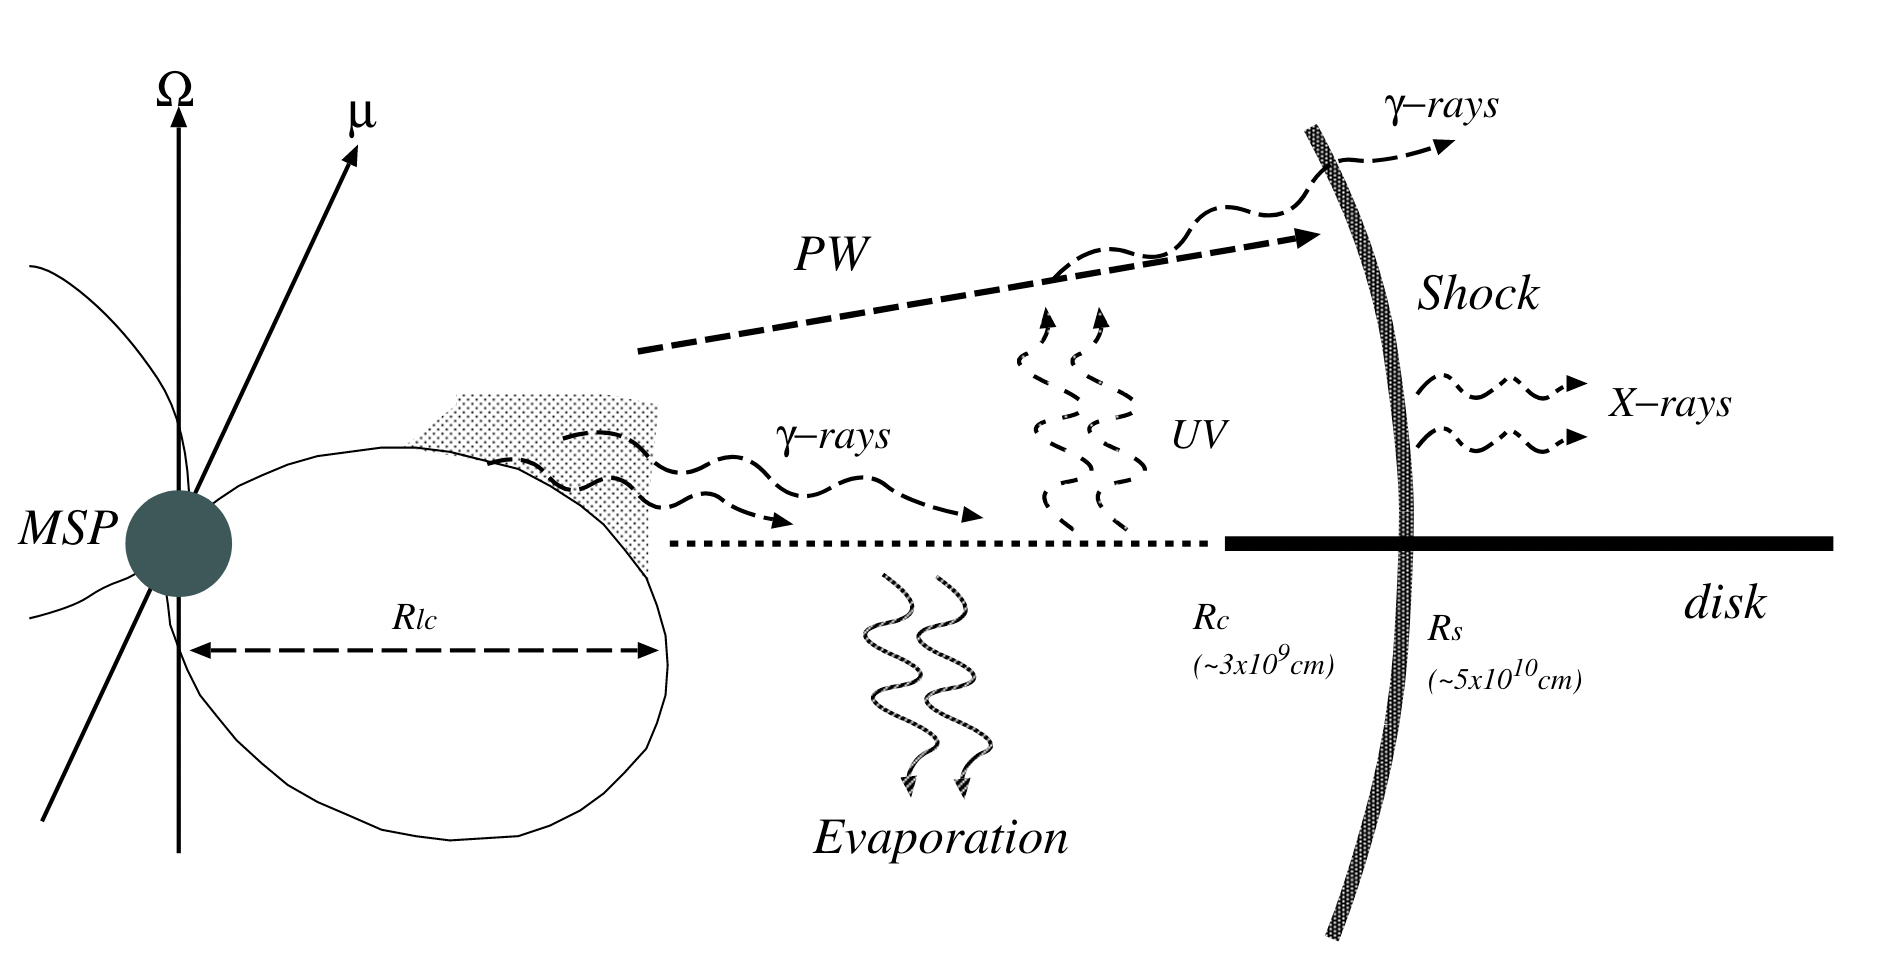
\includegraphics[width=0.8\textwidth]{figs/theory/redback-multiwavelength-emission.jpg}
    \caption{Figure taken from \cite{takata_multi-wavelength_2014}. Example of multiwavelength emission from a Redback pulsar.}
\end{figure}

It is thought that most milisecond pulsars are formed through the accretion of matter from a evolved compact binary system, the $\sim 30\%$ found in isolation are thought to have ablated their companion star to the point of dissapaction (citation). Matieral being thrown off the pulsar causes the radio emission to be eclipsed via scattering and absorption, for a segment of the companion's orbit. Rebacks systems exhibit both positive and negative period derivatives that are larger than the expected gravatiational radiation and is thought to a-rise from the interaction of the companion's magnetuc field and the pulsar's wind (citation). \\
Redback pulsars have been observed in two transional states ablation and accretion states (citation). These states are on sub year timescales. The transition in stages sees the magnitude of optical emission to increase by about $\sim 1$ order of magnitude. Studying optical emission from redback pulsars informs on the heating of the companion. Roche-lobe filling fraction and the mass of the system (citation). \\ Black widow pulsars have been observed to have little to no observable X-ray emission (citation). However, redaback's have been shown to exhibit much more x-ray emission in their thermal spectra with consistent double peaks obseravble when the pulsar is at inferior conjunction (citation). \\
The observed companions of redbacks are mostly faint stars with tempertures around X on the farside of the star from the pulsar. The companion's interaction with the pulsar dominates the thermal spectrum of spider pulsars from the present heating between the two. \\
X-ray emission from redbacks shows hard X-ray spectra that follows a power law with photon indices $(\Gamma)$ around 1 - 1.3. The energy of the thermal spectra in the X-ray is higher than what is expected from shock acceleration. Some models suggest tgat a wind-wind shock betweeb the pulsar and companion. However, this approach would require the wind momentum of the pulsar to be much weaker than the companion's. But similarly with the optical emission, the X-ray emission may be influenced by the magnetic field of the companion.  

\subsection{Why study Redback Pulsars?}

Redback pulsars have a number of interesting science cases. Redbacks undergo a range of phenomena, including radio and X-ray pulsations, accretion processes, and periodic eclipses as the companion star passes in front of the pulsar. Their study also provides valuable insights into the evolution of binary systems, the behavior of pulsars, and the physics of accretion processes.. Due to their transitional nature they provide a glimpse into the evolution of pulsars in the latter stages of their evolution. Pulsars are also used as tools to study theories of gravity, the interstellar medium and probe for gravatational waves. 

\subsection{Other exotic transients}

Redbacks themselves exotic transients, but there are many other clases of radio exotica that are of interest for the community. In this project work has also been carried out on an array of various radio transients and related objects. This includes the search for extraterrestrial intellgience (SETI), the study of M and Brown dwarf radio flares and the probing of potential radio emission from exoplanets. 

\subsubsection{Dwarf Stars}

\subsubsection{SETI}

The search for life elsewhere in the universe as always been a burning question for many astronmers throughotu history, even more the previlance of intellgient life in the universe. Since the 1960's there has been consisent surveys, mainly in radio that look for signals of artifical origin, commonly referred to as technosignature. These signatures are thought to be similar to that of radio signals produced artifically on Earth. These signals are mainly thought to be narrowband drifiting radio emission that would be produced by a transmitter leaking into space. To date there has been no positive detection of a technosignature. Similar to dark matter searches, the lack of detections has allowed for limits to be placed on the number of previlance of civilizations in the galaxy.

\begin{equation}
    N = R_* \cdot f_p \cdot n_e \cdot f_l \cdot f_i \cdot f_c \cdot L
\end{equation}


% \subsubsection{4FGL J0523-2529}

% \subsubsection{4FGL J2054-6904}
\newpage
\setcounter{page}{1} % only for draft purpose to keep page count on track
\section{Pulsar Searching in a Binary System} \label{sec:method-pulsar-searching}

As outlined in \cref{sec:prelude} the study of redback pulsars has a multitude of science cases. However, the number of known redback is small, in searching for new redback pulsars allows for further inquiry into the nature of the subclass. The search usually begins with the selection of potential candidates from large-scale surveys carried out by optical, X-ray and $\gamma$-ray observatories. Candiates are determined based on the flaring exhibted at these shorter wavelengths, then followed up using radio telescopes. Work to date has been to perform follow-up radio observations of Redback candidates to attempt to confirm radio emission and further compliment prior multiwavelength studies. \\ 

The \textit{Fermi} Large Area Telescope (LAT) provides the most candidates as the related $\gamma$-ray emission are not subject to the same limitations as other detection methods \citep{ray_radio_2012}. Both candidates observed so far as part of this project are two Fermi candidates 1FGL J0523.5-2529 and 4FGL J2054.2+6904. 

\subsection{Observation Campaigns}

J0523 was the first observed candidate and was observed using the Ultra-Wide-Bandwidth, Low Frequency Reciver (UWL)\footnote{The UWL operates from 704 to 4032 MHz (40 - 7 cm)} on the Parkes Murriyang telescope in New South Wales. Published studies from \cite{strader_1fgl_2014} and \cite{halpern_luminous_2022} provide the orbital period, companion's radial velocity and distance measurements for the system. Each of these factors are important in determining the observation and search strategy. \\ 

For the pulsar to be detected the radio emission from the poles must be visible to the observer plane of view and the beam must be unobsured by the companion star. The orbital phase can be easily calculated from the periodic emission in the optical as demonstrated in \cref{fig: velocities} using the following equation, 

\begin{equation}
    \phi = \frac{t - T_0}{P_{\text{orb}}}
    \label{eq: orbital phase}
\end{equation}

At the time of writing 74\% of the orbital phase has been observed, with time approved to observe the remaining orbital phase if the pulsar is not detected. \\

In the case of J2054 less information is known with no accurate phase ephermeris avalible. A study by \cite{karpova_new_2023} reports the period, companion radius and distance. Over 8 hours of observations have been carried out using I-LOFAR. In this case the entire orbit needs to be covered and blindly searched for radio emission within expected parameter range of a Redback pulsar. Observations with X are planned to take place in the Summer of 2024 to try and determine the orbital phase based. 

\begin{figure} %[h!]
    \centering
    \subfloat[\centering]{{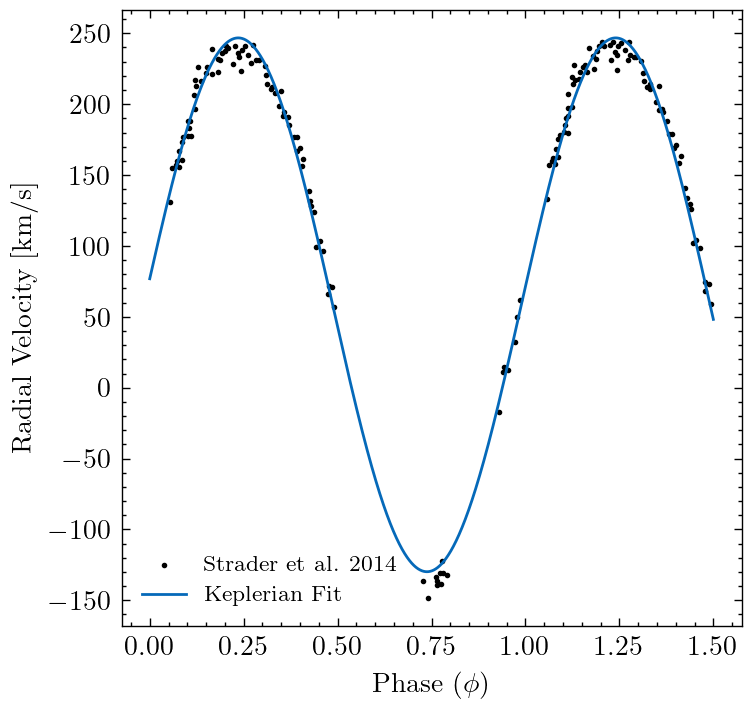
\includegraphics[width = 0.46\textwidth]{figs/radial-velocity.png}}}%
    \qquad
        \subfloat[\centering ]{{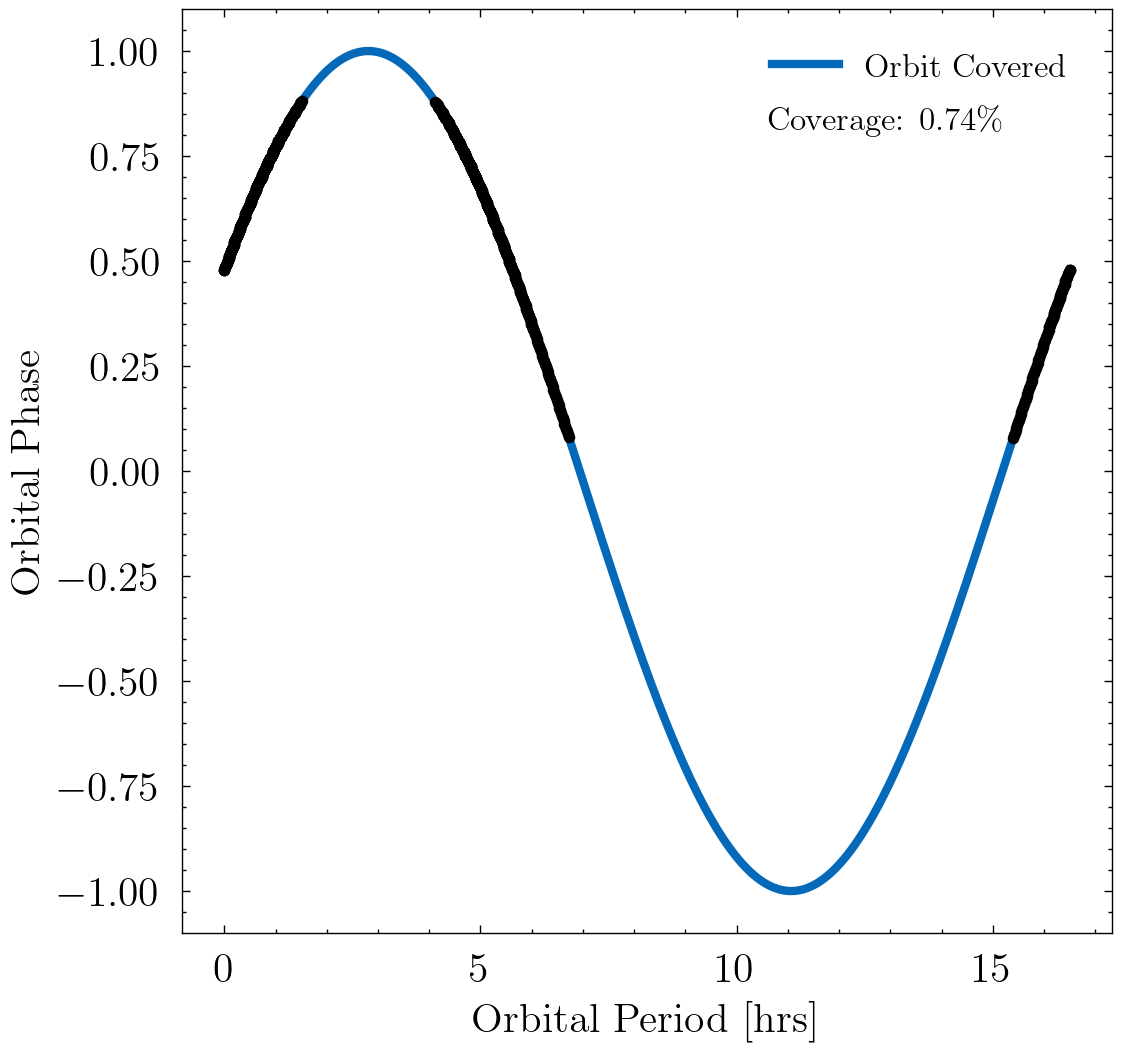
\includegraphics[width=  .46\textwidth]{figs/sine-wave-coverage.png}}}%
    \caption{\textit{(a)} Phased radial velocities observed from the optical counterpart of J0523 with the Keplerian fit overplotted. \textit{(b)} Observed oribital phase of J0523 with Parkes UWL to date. }%
    \label{fig: velocities}%
\end{figure}

\subsection{Observation Data} \label{sec:method-observation-data}

Observations from radio telescopes typically includes measurements of intensity, frequency, polarization and time. The data is usually stored in a time series format with the intensity and frequency measurements recorded at each time step. The data is usually stored in a  filterbanks (\texttt{.fil}) or .fits file format. The raw voltages are recorded and then processed into usable Stoke I files. 

\subsection{Search Strategy}

A zoo of pulsar software has been developed over the past decades to detect and time pulsars. One of the most commonly used softwares in the search for binary pulsars is PRESTO \citep{ransom_new_2001}. The search is carried out as illustrated in \cref{fig: presto-work-flow} and due to the large data volumes produced by modern telescopes, the search is carried out in a distributed manner on high performance computing clusters. \\ 

\begin{figure}
    \centering
    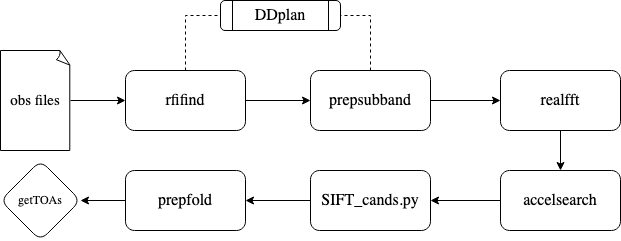
\includegraphics[width = 0.9\textwidth]{figs/presto-work-flow.drawio.png}
    \caption{Outline of the PRESTO search strategy used to search for binary pulsars.}
    \label{fig: presto-work-flow}
\end{figure}

\subsubsection{RFI Removal}

The first step in nearly all radio observations is to remove Radio Frequency Interference (RFI) from the observations data, this is usually caused by most modern technologies. This is important as artifical signals can mimic period signals associated with pulsar emission. Thus the data must mask frequencies or be clipped in the time domain. This project makes use of \texttt{rfifind} to remove such RFI. 

\texttt{rfifind} which is part of the PRESTO suite searches in both frequency and time domains. It analyses each channel for a specified time integration. Firstly the time domain statitics are computed which consists of the mean and stadared deviation of the values in each channel. For blocks where the mean value exceeds $4\sigma$ the block is flagged as RFI. If more than 30\% of the channel is flagged the entire channel is masked completely and replaced with a median constant bandpass value. An example of a mask produced by \texttt{rfifind} is shown in \cref{fig: rfifindexample}. 

\subsubsection{Incoherent Dedispersion}

Following the masking of all observation files the next step is to inchoherently dedisperse the data. This is done to remove the effects of dispersion caused by the interstellar medium as discussed in X. Failure to de-disperse data broadens potential pulse profiles and significantly reduces the signal to noise ratio. \Cref{fig: DM_pulse_example} shows an example of pulse dispersion. Inchoherent dedispersion is carried out by splitting the data into subbands and then shifting the data in time to correct for the desipersion. 


\begin{figure}
    \centering
    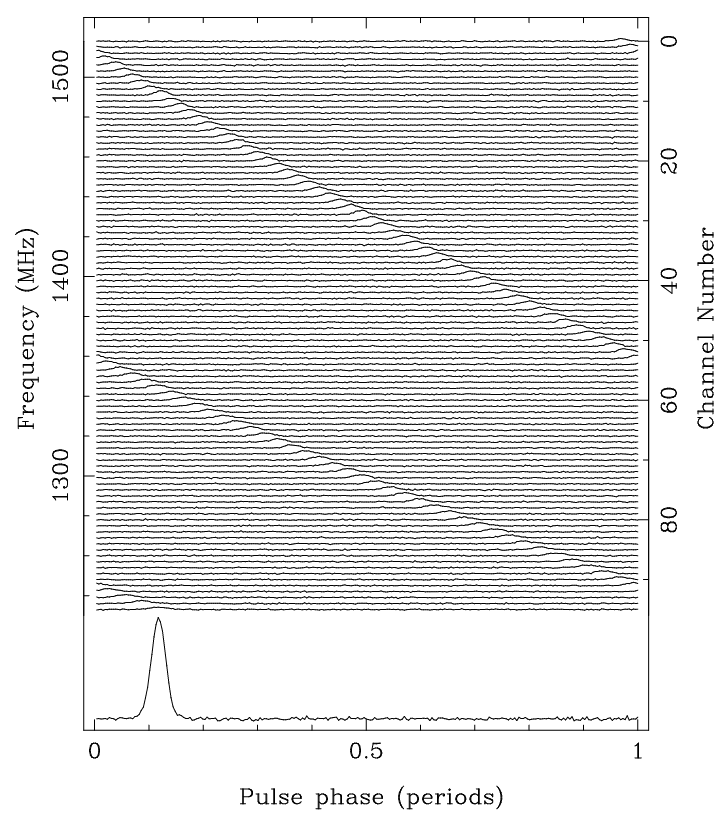
\includegraphics[width = 0.6\textwidth]{figs/DM_pulse_example.png}
    \caption{Example of a dispersion pulses of 128 ms pulsar B1356-60, which has a dispersion measure of 295 pc cm$^{-3}$. Figure from \citet[p.~20]{pulsar_handbook}.}
    \label{fig: DM_pulse_example}
\end{figure}

When correcting for dispersion it is important to consider the possible range of DMs that the pulsar could exhibit. The DM can be estimated through the use of density electron models such as X and X. However when dedisperseing the data it inherently induces smearing in the data. There are four types of smearing that need to be acounted for and characterized by the following equation, 

\begin{equation}
    \tau_{\text{total}} = \sqrt{\tau_{\text{samp}}^2 + \tau_{\text{sub}}^2 + \tau_{\text{BW}}^2 + \tau_{\text{chan}}^2}
\end{equation}



\begin{figure}
    \centering
    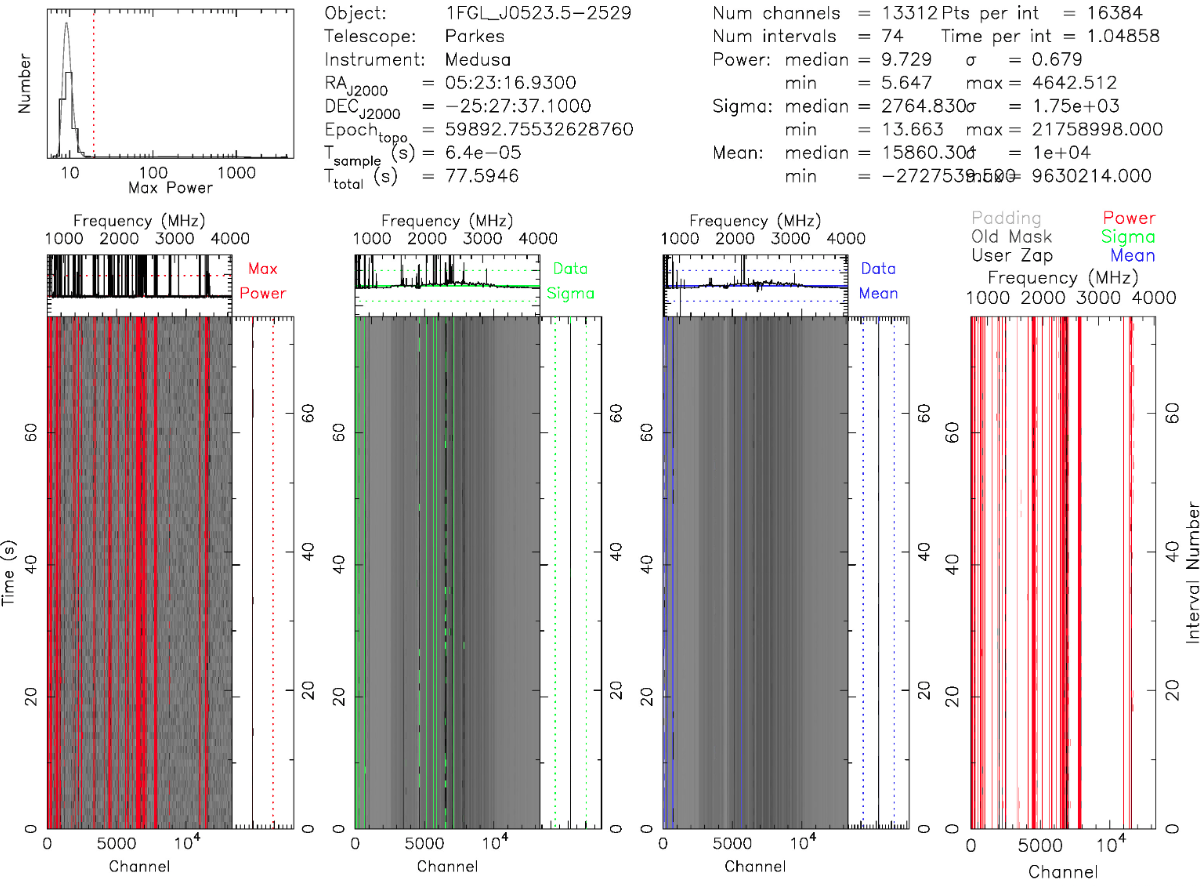
\includegraphics[width = 0.8\textwidth]{figs/rfifindexample.png}
    \caption{Example of RFI removal using \texttt{rfifind} on a 77 second observation of J0523. The upper left panels shows the max power profile of the RFI detected. The bottom most left panel show the max power, the second panel to the right shows the $\sigma$, the third panel shows the mean and the right most panel is the reccomended mask with all panels plotted.}
    \label{fig: rfifindexample}
\end{figure}

\subsubsection{Fast Fourier Transform}

The data is needs to be transformed into the frequency domain to search for periodic signals. This is commonly done with a Discrete Fourier Transform (DFT) in pulsar astronomy and computationally carried out using a Fast Fourier Transform (FFT). For a time series, $S_j$ of a given length of $N$ it is neccessary to convert the time series into the barycentric frame of reference. The barycentric frame if reference point is centered on the mass of the solar system. \\ The $k$th Fourier component of the time series is described in \citet[pp.~132-134]{pulsar_handbook} as,

\begin{equation}
    \mathcal{F}_k = \sum_{j=0}^{N-1} S_j \exp\left(-2\pi \sqrt{-1} \frac{jk}{N}\right)
\end{equation}

To complete this computation it requires $N^2$ floating point opearations. However, if a FFT operation is employed the number of operations is reduced to $N \log_2 N$ for a time series of length $N$. Since the time series data are real numbers symmetry can be exploited as the DFT is symmetric about the Nyquist frequency, $\nu_{\text{Nyq}} = 1/(2 t_{\text{samp}})$. For any frequencies higher than the $\nu_{\text{Nyq}}$ the complex conjucate is the same as the corresponding lower half of the frequency.

On the software side this is carried out with the \texttt{realfft} function in PRESTO. This result intakes the dedisperesed subbands and returns the power spectrum of the data. At this point the data is in a state to be searched for periodic signals.

\subsubsection{Accelration Searching}

Searching for binary pulsars requires a slightly different approach as the motion of the system causes the observed pulse frequency to smear across the Fourier bins (Cherry's paper), in turn this reduces the sensitivity of the search. A solution to this is to split up the search into smaller time intervals and assume that the radial velocity is a constant on this time scale. This can be shown to be a good approximation for $P_b/10$. \\ 
The spin frequency, $f_{\text{spin}}$ and the time of pulse emission, $t_{\text{pulse}}$ the pulsar's phase can be expressed as, $\phi_p = f_{\text{spin}}t_{\text{pulse}}$. Morever, the pulse time can be expressed as the time of arrival from the pulsar, $d(t_0)$, 

\begin{equation}
    t_{\text{pulse}} = t_0 - \frac{d(t_0)}{c}
\end{equation}

thus the phase can be expressed as,

\begin{align}
    \phi_p = & f_{\text{spin}}\left[ t_0 - \frac{d(t_0)}{c}\right] \\ 
    = & f_\text{spin} \left[ t_0 - \frac{a \sin i}{c} \sin \left[ \frac{2 \pi (t - t_{\text{asc}})}{P_B} \right] \right]
\end{align}

where $a$ is the semi-major axis, $i$ is the inclination angle, $t_{\text{asc}}$ is the time of ascending node and $P_B$ is the orbital period. A Taylor expansion can be used to $\sin x$ around $x = a$ such that, 

\begin{equation}
    \sin (x) \simeq   \sin (a) + \cos (a)(x - a) - \frac{\sin (a)}{2!}(x - a)^2 - \frac{\cos (a)}{3!}(x - a)^3 + \ldots
\end{equation}

Therefore the phase of the pulsar with a constant spin down rate can be expressed as, 

\begin{equation}
  \phi(t) = f^1 t_0 + \frac{\dot f}{2} (t - t_0)^2 + \frac{\ddot f}{6} (t - t_0)^3 + \ldots 
\end{equation}

Matching co-effcients between the the full Taylor expansion and the phase expression for the pulsar gives the following relation, $\dot f/2 = f_{\text{spin}} \frac{a \sin i}{c} A$. Where $A$ is represents all the terms in the expansion. The final simplified expression works out to be, 

\begin{equation}
    \dot f = f_\text{spin} \frac{4 \pi^2 a \sin i }{cP^2_B} \sin \left[ \frac{2 \pi (t - t_{\text{asc}})}{P_B} \right]
\end{equation}

Thus over a small enough time period spin-down is approximately constant.

\begin{equation}
    \frac{k_2 P_B}{2 \pi q} = a \sin i   
    \label{eq:constant_accel}
\end{equation}

Where $k_2$ is the radial velovity semi-amplitude, $P_B$ is the orbital period and $q$ is the mass ratio.

Searching is carried out using \texttt{accelsearch} which searches the FFT time series for period emissions by summing the highest Fourier frequency derivative. The number of bins that this signal is smeared is given by the acceleration parameter \citep{ransom_new_2001}, 

\begin{equation}
    z \simeq \dot f T^2_{\text{obs}}
\end{equation}

Where $T_{\text{obs}}$ is the length of the observation. The search is carried out over a range of accelerations which can be based on \cref{eq:constant_accel} if the physical quantities are known. A list of the known orbital parameters for the two candidates is given in \cref{tab:orbital-parameters} along with resultant z values.
 
\begin{table}[H]
    \centering
    \begin{tabular}{c|cccccc}
        \hline
        Candidate & $P_{\text{orb}}$ (days) & $k_2$ (kms$^{-1}$) & $a \sin i$ (s) & $e$ & $q$ & z\\
        \hline
        J0523.5-2529 & 0.68813 & 190.3 & 0.359 & 0.040 & $0.61 \pm 0.06$ & \\
        J2054 &  &  & & & & \\
        \hline \hline 
    \end{tabular}
    \caption{Orbital parameters of the two candidates. Values for J0523 are taken from \cite{strader_1fgl_2014} and \cite{halpern_luminous_2022}. Values for J2054 are taken from \cite{karpova_new_2023}.}
    \label{tab:orbital-parameters}
\end{table}

In cases where the orbital parameters are not known the search is carried out over a range of accelerations from 0 to 200, and even in the case where the value exceeds 200, this is left as a cap on the search. The reason that the search is not carried out over the entire range is due to the computaitonal cost and is often not neccessary with accelerations above 200 starting to exhibit a non-linear relationship as stated in \citet{ransom_new_2001}. Once the search is carried out the results are outputted in the form of candidates with estimates on DM, S/N, period and frequecies. 

\subsubsection{Folding and Timing}

Pulsar folding is a technique commonly used when the pulses are not bright enough to be clearly visible in the observed time series. The term folding comes from the fact that the time series is folded on itself by some trial period of the pulsar, this is illustrated in \cref{fig: folding}. 

\begin{figure}
    \centering
    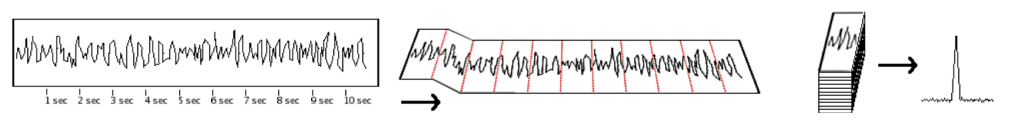
\includegraphics[width = 0.9\textwidth]{figs/folding.png}
    \caption{Adapted illustration from X of the folding process. The left panel shows the observed time series, the middle panel shows the folded time series and the right panel shows the summed pulse profile.}
    \label{fig: folding}
\end{figure}

Using a routine called \texttt{prepfold} each of the candiates over the noise floor are folded with each candidate examined by eye for possible postive pulsar detection. An example of this is shown in \cref{fig: prepfold}. This plot contains integrated pulse profile, time series plot and subband plot. It also shows DM, $P$ and $\dot P$ plots as a function of reduced $\chi^2$ values. 

\begin{figure}
    \centering
    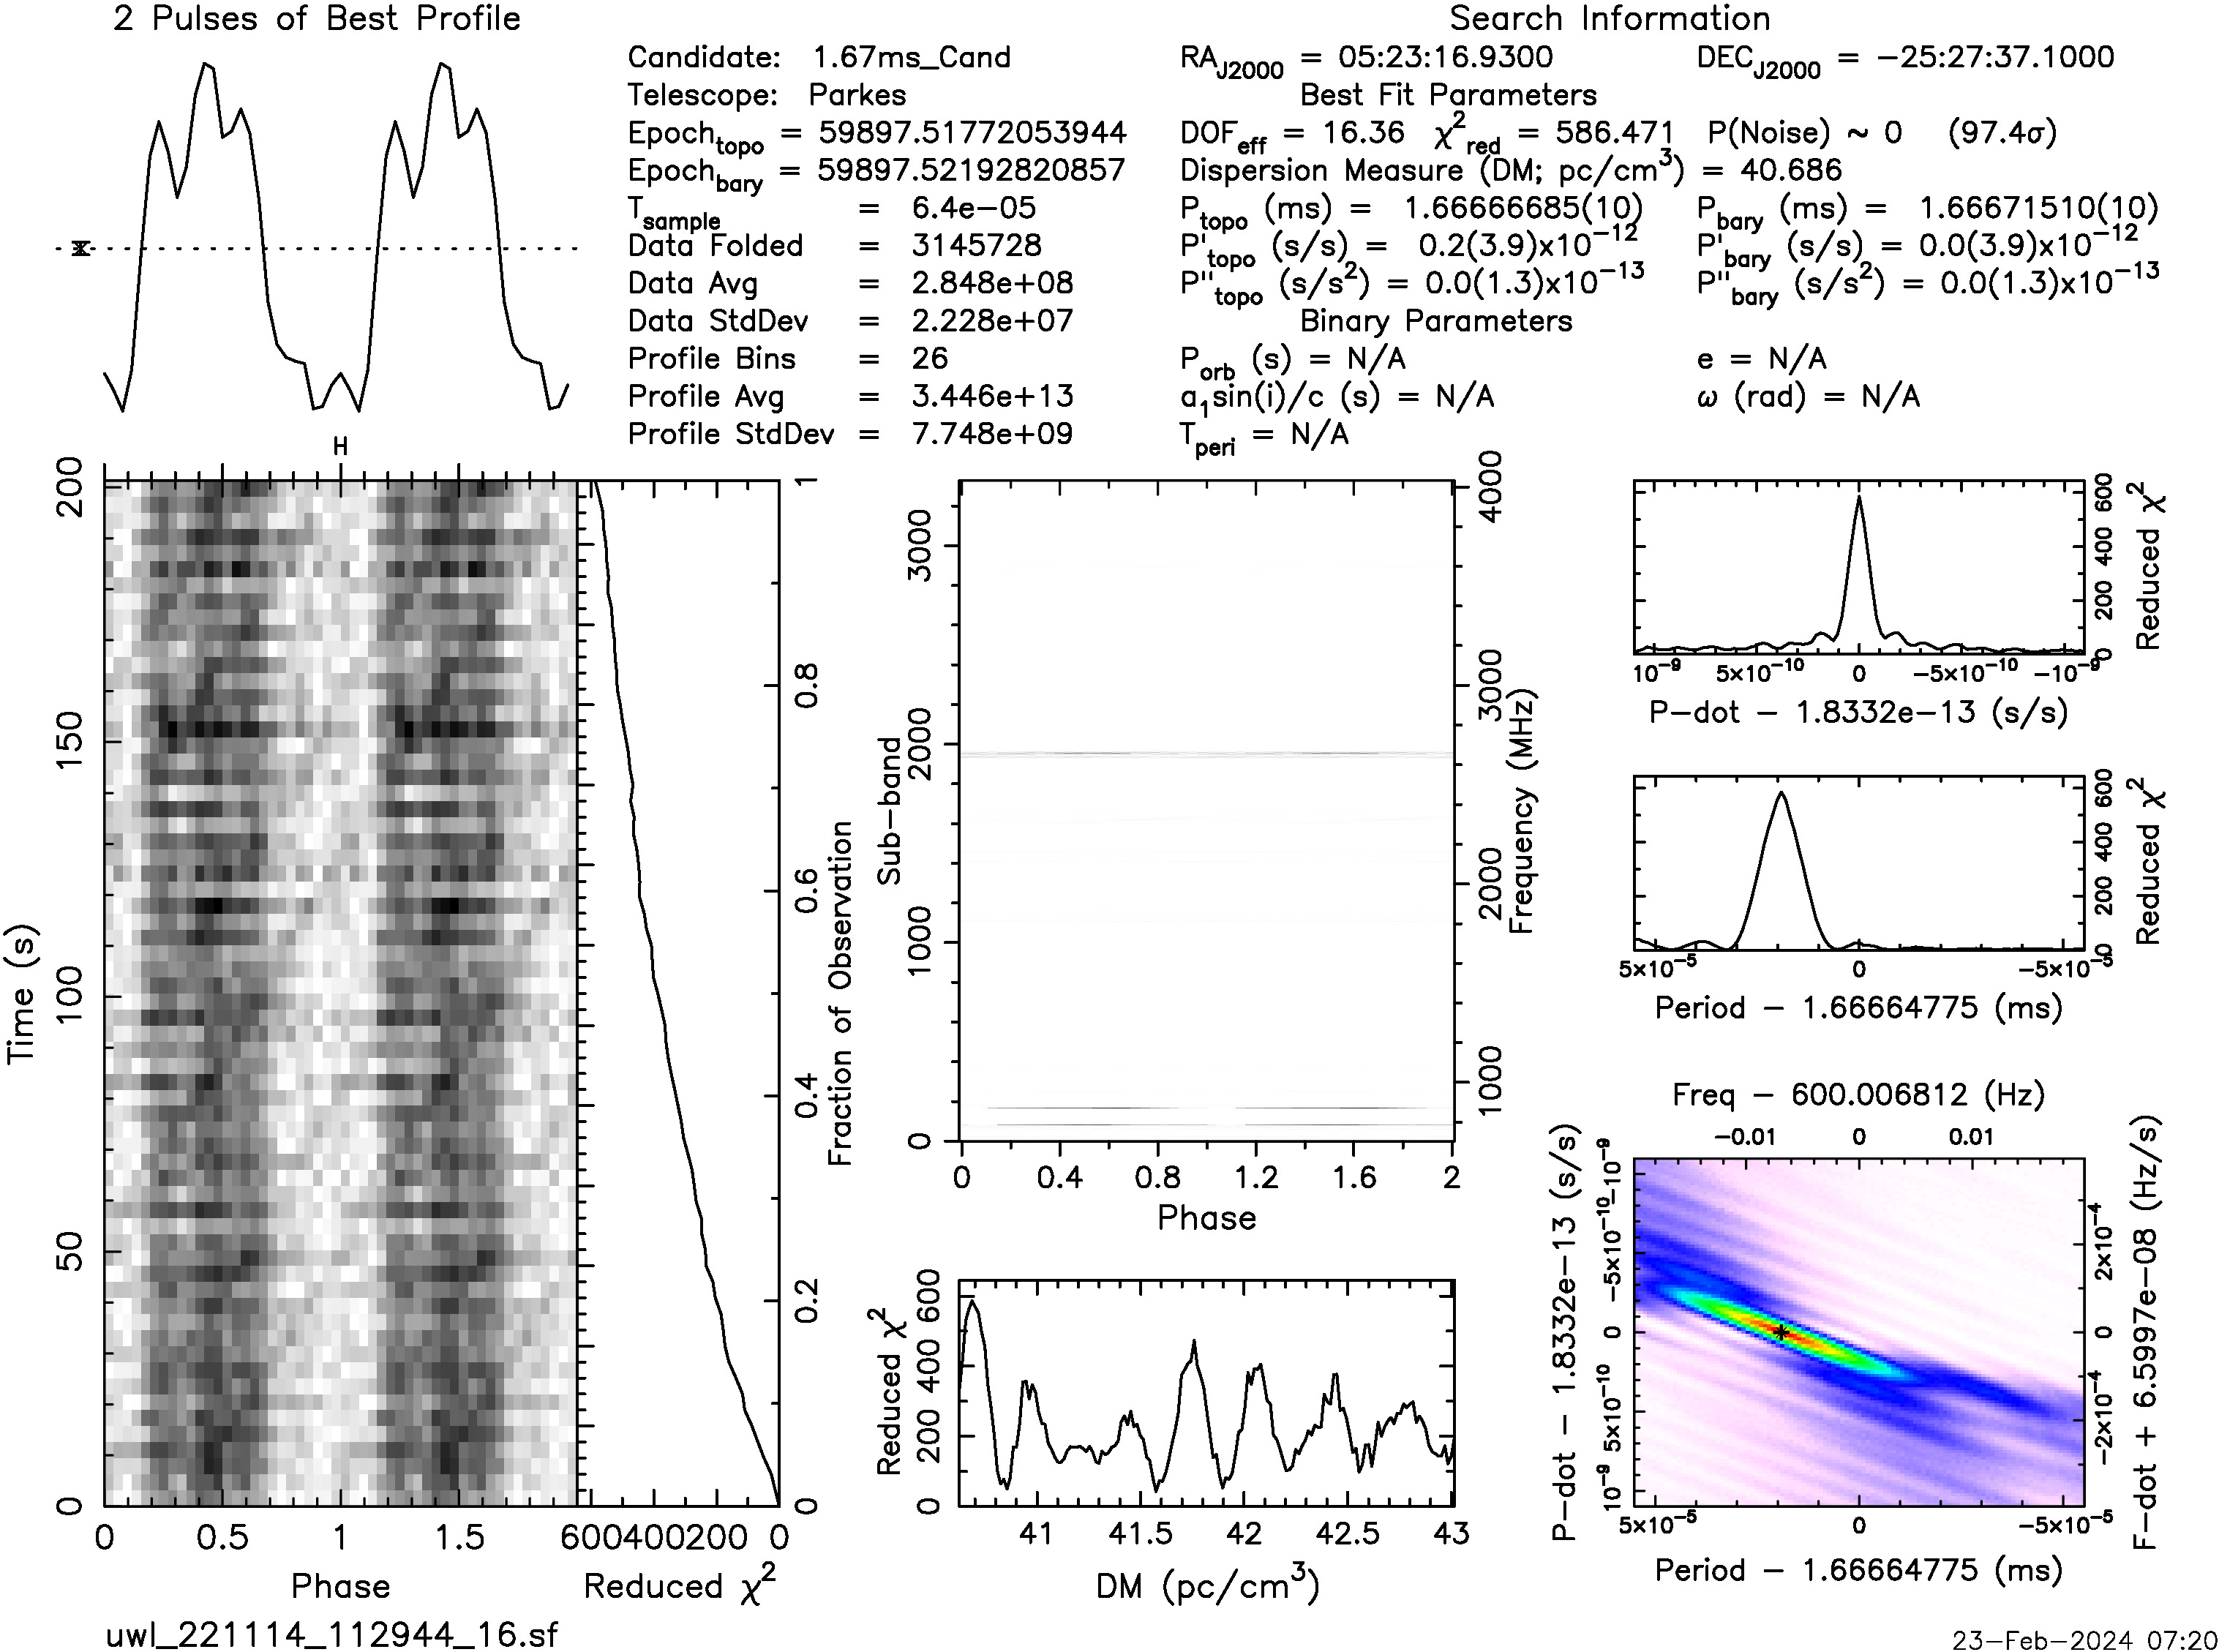
\includegraphics[width = 0.9\textwidth]{figs/prepfold.png}
    \caption{Example of a \texttt{prepfold} plot for a candidate.}
    \label{fig: prepfold}
\end{figure}

\section{Technosignature Searches at Low Frequencies} \label{sec:method-technosignature-searches}

The first year of the project primarly entailed the publication \citep{johnson_simultaneous_2023} of results from the first search for technosignatues at low frequency using Irish and Swedish LOw Frequency ARay \citep[I-LOFAR;][] {van_haarlem_lofar_2013}. When carrying out this technosignature search the two main goals were to constrain the prevalance of intellgient civilizations in the Milky Way at an unexplored frequency and use the collected data to search for other exotic transients such as Fast Radio Bursts (FRBs), pulsars, magnetospheres and M-dwarf emission \citep{sheikh_nine_2020}. 

\subsection{LOFAR}

LOFAR, a pioneering low-frequency aperture array telescope, spans hundreds of kilometers across Europe and serves as a pathfinder to the Square Kilometer Array (SKA). The array consists of a core station with outrigger stations situated in the Netherlands and additional international stations spanning multiple countries, such as Germany, France, Sweden, Ireland, Latvia, Poland, and the United Kingdom. Additionally, stations are currently in the process of being constructed in Italy and Bulgaria. The LOFAR array operates using two types of antenna, the Low Band Antenna (LBA) and the High Band Antenna (HBA), operating at 10–90 MHz and 100–250 MHz respectively. In this study, the HBAs at the Irish and Swedish LOFAR station are used to carry out observations noninterferometrically. The field of view (FoV) of an international LOFAR station is rather large; at full width at half maximum, it is 5.3, 3.4, and 2.3 deg$^2$ at frequencies of 120, 150, and 180 MHz, respectively \citep{van_haarlem_lofar_2013}. The station is capable of resolution of 3.3 and 0.2 arcsecond at the bottom and the top of the bad respectively when the entire array is in use making it one of the most sensitive telescopes in the world.

\subsection{Target Selection}

% Observation campaigns for this survey were carried out through the Summers of 2021 and 2022. Targets were selected for the survey based on exoplanet candidates from NASA's Transiting Exoplanet Survey Satellite \citep[TESS;][]{TESS2015}. In modern technosignature survey's the choice of exoplanet's surveyed is indifferent to characterstics of exoplanet and host star. This decision is due to the limited knowledge of ideal life harbouring conditions a planet must have. Instead the survey opts for sensitivity. Thus, targets were selected based on their distance ($\leq 1$ kpc) and altitude during time of observation. In total 44 TESS targets were observed \citep[see Table 2][]{johnson_simultaneous_2023}.

A significant fraction of radio emission from Earth is emitted in the direction of the ecliptic plane. For example, powerful planetary radars are used to explore Solar System objects \citep{Siemion_KEPLER_ApJ}, and high-powered transmitters are used to communicate with Solar System probes \citep{Enriquez2017ApJ}. It is conceivable then that such leakage radiation may also be emanating from other worlds, preferentially in their planetary orbital planes. This is why we chose TESS targets, as these are the closest transiting exoplanet systems known \citep{Kepler_Mission_Design_2010,TESS2015}. Observing these sources with the LOFAR HBAs enables robust constraints on any associated artificial low-frequency radio emission

\subsection{Expanding the Cosmic Haystack}

Searching for technosignatures is akin to searching for a needle is a cosmic sized haystack. The beam of a LOFAR station has an expansive coverage enabling observation of a substantial number of stars in the field of view. The significance of these in-field stars has been highlighted by \cite{Bart-Wlodarczyk-Sroka}. Consequently, during our observations targeting 44 sources from the TESS catalog, we encountered a significant number of in-field stars within our field of view, as shown in Figure 2. \ 
To determine the list of targets within this field of view, we utilized the Gaia catalog. Some previous major SETI surveys focused their searches toward Sun-like stars \citep{Tarter:1996jf}. However, because our understanding of the origin of life is limited, it makes sense to allow for the possibility of life arising on a planet that is neither Earth-like nor around stars that are Sun-like. Similarly, we should consider planets not necessarily located in the habitable zone. This is typically characterized as the orbital range wherein liquid water could exist \citep{Kasting1993}, as inferred from planetary equilibrium temperatures often ignoring the unknown albedo of the exoplanets. Any sensitive radio SETI survey seeking to maximize the chance of detecting weak radio signals should, insofar as possible, expand its search to encompass nearby stars of a broad range of spectral types and with exoplanets of all sizes and distances from their parent star. Thus, we conducted calculations to determine the number of Gaia stars with a mean distance of 1215 pc, with an accuracy in their distances of at least 20\%. This study used Gaia's third data release \cite[GDR3;][]{GaiaDR3,astroquery}. When analyzing GDR3, two filters were applied to the survey volume and sensitivity accuracy of the in-beam target values. First, a constraint on the R.A. and decl. errors was implemented. If a Gaia source was found to be in the beam but had an error magnitude greater than the FWHM, it was removed from the source pool. \Cref{Gaia:filter1} states the first condition of filtering:

\begin{equation}
    \theta_{\text{sep}} + \sqrt{\Delta \text{RA}^2 + \Delta \text{Dec}^2} \leq \frac{\text{FWHM}}{2}
    \label{Gaia:filter1}
\end{equation}

As the sensitivity of the survey is calculated based on a source's distance, a second filter is implemented to remove sources that have large errors. By taking the difference $(\Delta \sigma_G)$ in the upper and lower confidence levels of GSP-Photometry, we obtain a percentage error on distance. All sources with a $d_{M_G}$ error of 20\% or greater are filtered out of the source list. \Cref{Gaia:filter2} states the second condition of filtering:

\begin{equation}
    \frac{\Delta \sigma_G}{\sigma_G} \leq 20\%
    \label{Gaia:filter2}
\end{equation}

A total of 1,631,152 stars form this list, making it one of the largest samples of stars ever surveyed for SETI purposes.

\subsection{Carrying out a Dual-Site Survey}

% Following the selection of targets the survey is carried out using a custom pipeline. The pipeline developed for carrying out this survey is detailed in \cref{fig:SETI-pipeline}. Narrowband technosignatures have a width of a couple of Hz thus high frequncy resolution is required. As similarly discussed in \cref{sec:method-observation-data} the raw voltages need to be dignitized using a suite of software. In this case \texttt{GUPPI RAW} and \texttt{RAWSPEC}

\begin{figure}
    \centering
    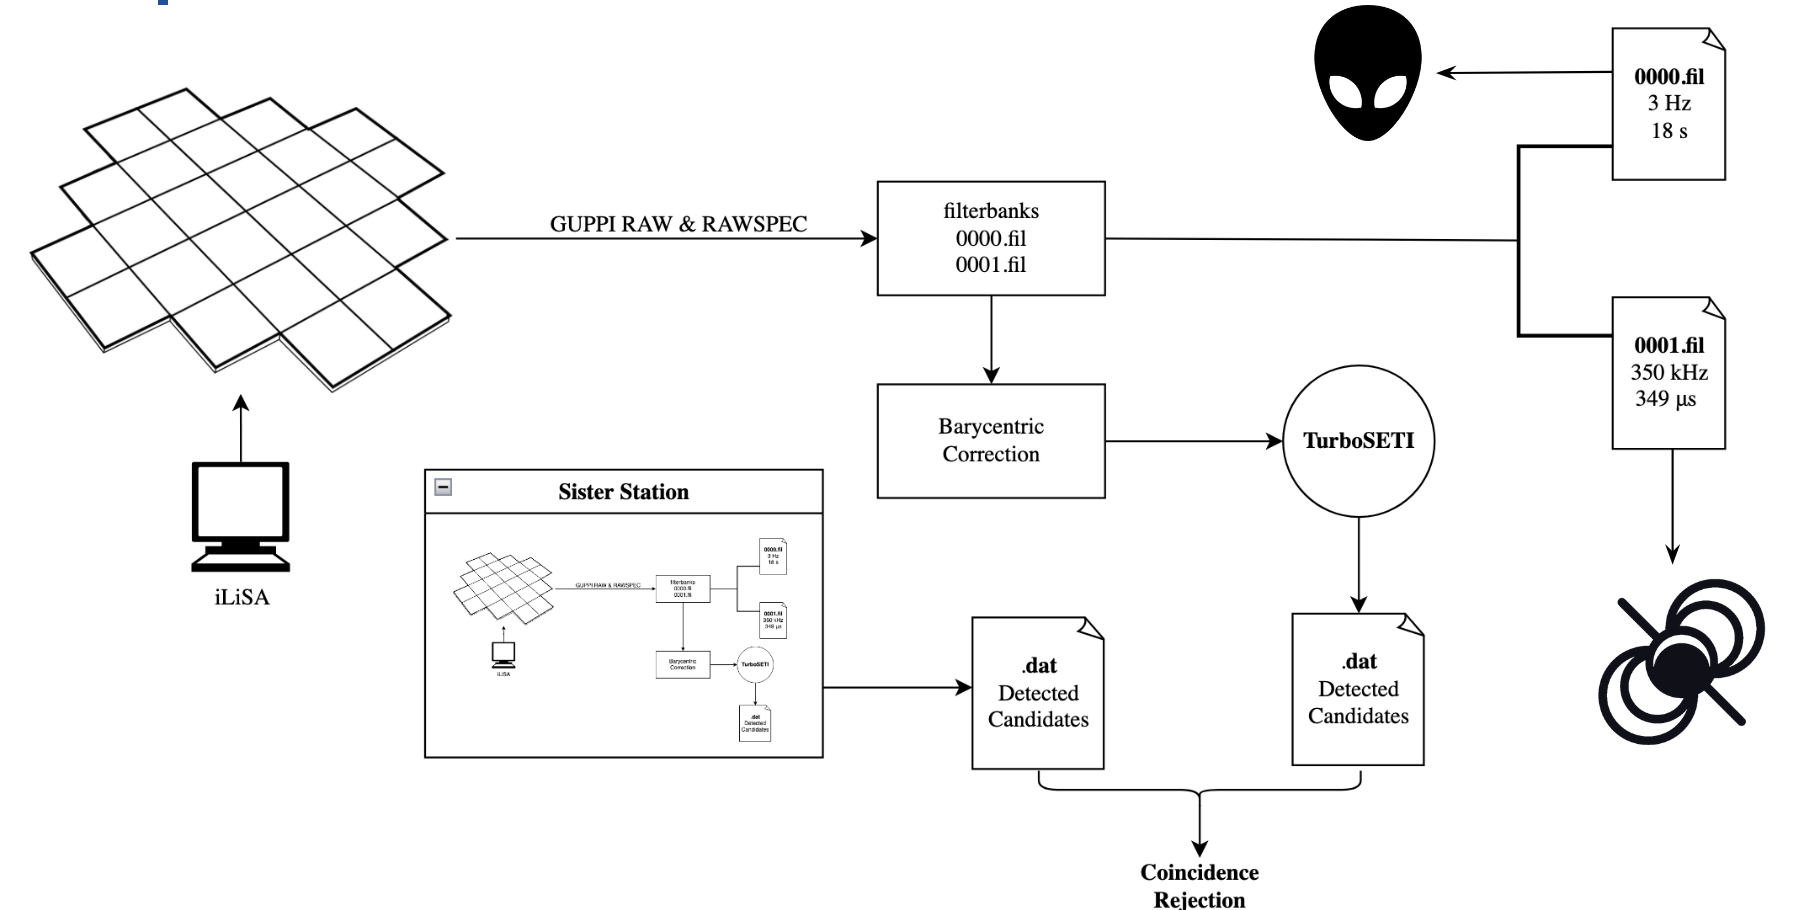
\includegraphics[width = 0.9\textwidth]{figs/SETI-pipeline.png}
    \caption{Outline of the SETI pipeline developed and deployed on Breakthrough Listen nodes at both LOFAR stations.}
    \label{fig:SETI-pipeline}
\end{figure}

Typically, international LOFAR stations operate as standalone telescopes $2-3$ days per week, i.e. they do not operate as part of the International LOFAR Telescope's Europe-wide array. This project was undertaken during this standalone time. For this purpose the \emph{international LOFAR in Stand-Alone mode} (\texttt{iLiSA}) package\footnote{\url{https://github.com/2baOrNot2ba/iLiSA/releases/tag/v6.1}} is used to control both telescopes simultaneously. \texttt{iLiSA} provides a high-level operational control of multiple LOFAR stations, including scheduling, processing pipeline dispatching and metadata aggregation. For the observations in this study, an operator-produced list of targets that were close\footnote{In practice as Birr and Onsala are separated by $\sim20\deg$ of longitude, the optimum scheduling is to observe $\sim 40$~min$-T_{\rm obs}/2$ `late' at Onsala and $40$~min$+T_{\rm obs}/2$ `early' at Birr.} to the local meridian was fed into \texttt{iLiSA} at each epoch. Towards each target, one beam per station was formed using \texttt{iLiSA}, and each beam was formed with $412$ HBA sub-bands (corresponding to a bandwidth of $80.46875$~MHz). The scan time on each target was $15$~min, and the whole scheduling block was a few hours per epoch. \ 
Data was preproccessed\footnote{For detailed explanation of the preprocessing and preperation see \cite{2019_Lebofsky}} and prepared using the \texttt{udpPacketManager} package \citep{David_JOSS}. Which resulted in two sets of filterbanks for each observation, each with different frequency and time resolutions. The first set of filterbanks had a frequency resolution of $2.98$~Hz and a temporal resolution of $0.67$~s. The second set of filterbanks had a frequency resolution of $350$~kHz and a temporal resolution of $349~\mu \text{s}$. The first set of filterbanks was used for the search for narrowband technosignatures, and the second set was used for the search for broadband transients. \

\subsection{Narrowband Search Results}

Using \textit{turboSETI}, a Doppler-drift search was carried out on the observed candidates at both stations. This resulted in the list of “hits” collected, where hits are defined as a narrowband signal detected above the given threshold, S/N = 10. The distribution of narrowband signals detected at both stations is shown in Fig X. A large percentage of hits are seen at both sites in the 120-140 MHz range. This falls within the range of expected RFI leakage seen from neighboring airports\footnote{Shannon \& Goteborg Landvetter.}. \ 
Using a drift-rate search of $\pm 4 \ \text{Hz/s}$ for this study covers a fraction of the possible drift rates of transmitters from exotic objects that can be detected as outlined by \cite{Sheikh_2019}. \cite{LiNarrowBand} shows that 4~Hs/s is comprehensive in relative to the expected distribution of exoplanet drift rates. The omission of a search in this parameter space is due to its computationally intense nature of searching for narrow-band signals across a sizeable drift-rate range. However, in doing this, the parameter space searched for ETI signal has been drastically reduced. Continual development of search algorithms like \verb|turboSETI| is progressing to make larger drift-rates searches a more computationally feasible. \
Upon first inspection of \Cref{fig:hits-histogram} it appears that the results at both stations are somewhat similar. However, upon performing a Kolmogorov-Smirnov (KS) test for each set of results for drift-rate, SN and frequency of detected hits the highest $p$-value returned was on the order of $10^{-11}$ indicating that the RFI environments at each of the stations are significantly different. \ 
In the case of this study, a singular beam observes a single target for 15 minutes at both stations and observations are converted to barycentric reference frame. Narrow-band searches are then performed at both sites, and the results of both searches are compared.

In our analysis, a signal is classified as a mutual extraterrestrial hit only if two conditions are met: \textit{a)} the signals are within a frequency range of $\pm 4 \ \text{Hz}$ of each other in the barycentric reference frame, and \textit{b)} their drift rates are within $\pm 0.2 \ \text{Hz/s}$ of each other after barycentric drift corrections. In Figure \ref{fig:barycentric correction}, an intriguing candidate is depicted. In the topocentric frame, we detected a narrowband signal at 160 MHz that was simultaneously present at both stations. However, when converting to the barycentric reference frame (as illustrated in Figure \ref{fig:barycentric correction}), the signal appears to be seen at different frequencies with opposite signs due to the different line-of-sight velocities towards the target. As a result, this narrowband signal is rejected as a genuine sky-bound signal.

\begin{figure} %[h!]
    \centering
    \subfloat[\centering]{{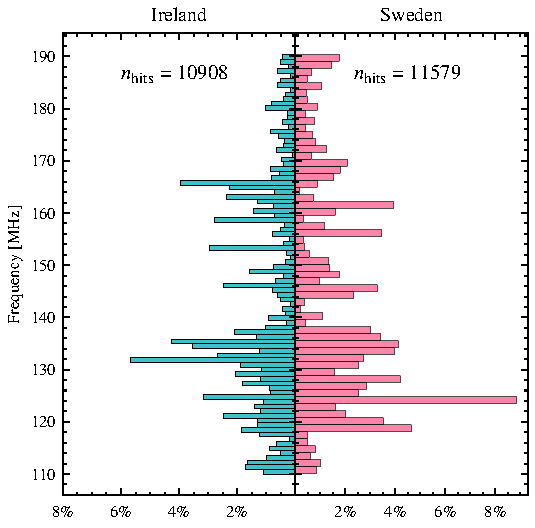
\includegraphics[width = 0.46\textwidth]{figs/hits_comparative_histogram.pdf}}}%
    \qquad
        \subfloat[\centering ]{{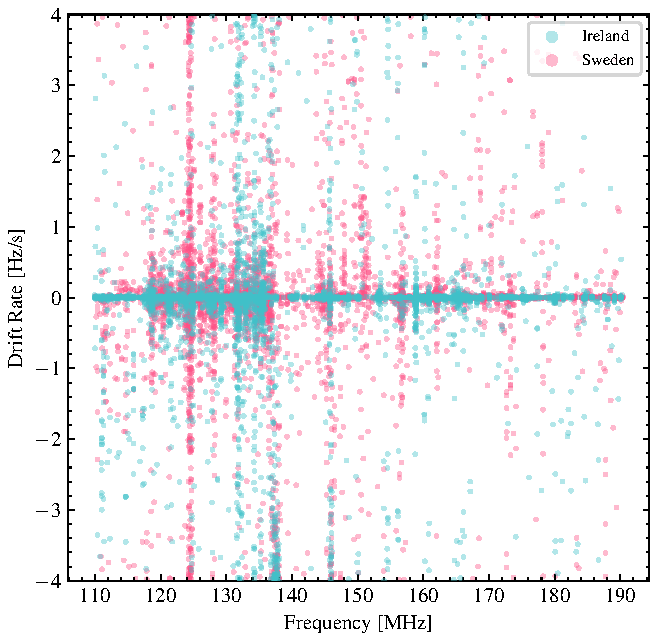
\includegraphics[width=  .46\textwidth]{figs/DR_scatter_plot.pdf}}}%
    \caption{\textit{(a)} Comparison of drifting signals or “hits” detected at both stations seen across the HBA frequency band. Each bin within the data set represents a 1 MHz frequency range and is accompanied by a corresponding percentage indicating its proportion to the overall data set. \textit{(b)} A scatter plot of the drift-rate values against detected frequency. The Irish station is shown in pink and the Swedish station is shown in blue.}%
    \label{fig:hits-histogram}%
\end{figure}

\subsection{Constraints placed by the Survey}
\begin{figure}
    \centering
    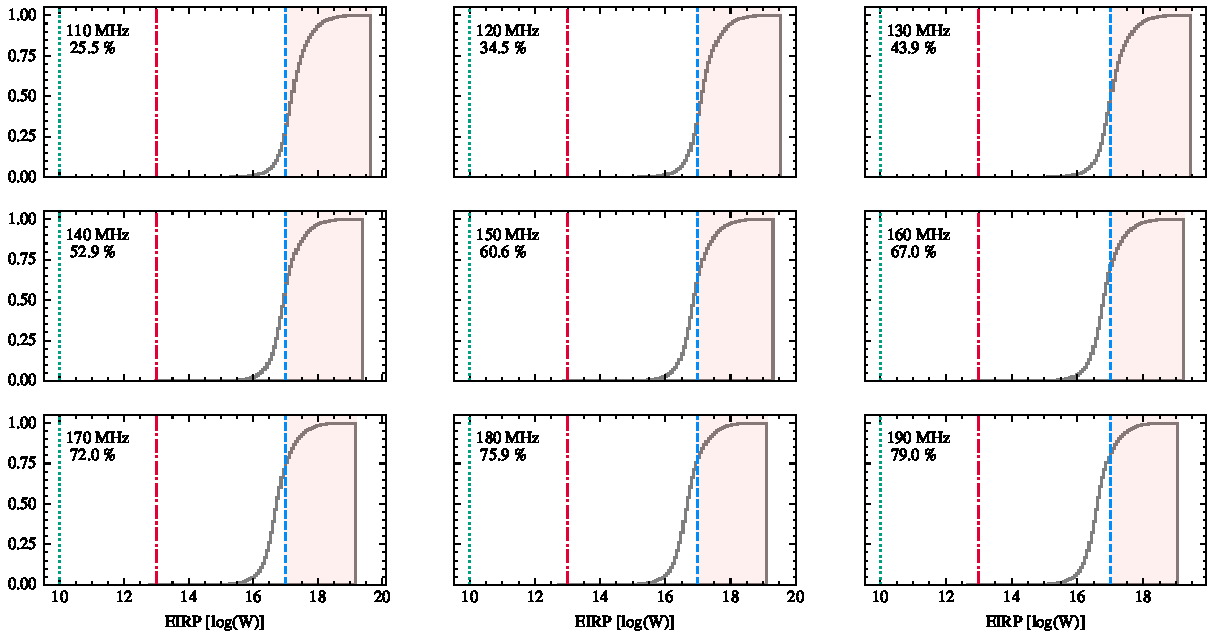
\includegraphics[width = 0.95\textwidth]{figs/EIRP_hist_plot.pdf}
    \caption{Cumulative histogram of EIRP limits of this survey across the HBA band. Reference luminosities for three civilization Kardeshev levels emitting $10^{17}$,$10^{13}$ or $10^{10}$ W are shown in blue, red, and green respectively. The percentage of targets where the station is sensitive to the transmission of $10^{17}$ W is shown, as a function of frequency across the band. At lower frequencies, sensitivity to $10^{17}$ emitters drops off as the $T_{\text{sys}}$ rises. The $\bar T_{\text{sys}}$ varies from 1260 K down to 322 K as frequency is increased across the band. Detailed calculations are presented in Appendix B of \cite{johnson_simultaneous_2023}.}
    \label{fig:EIRP-limits}
\end{figure}

\begin{figure}
    \centering
    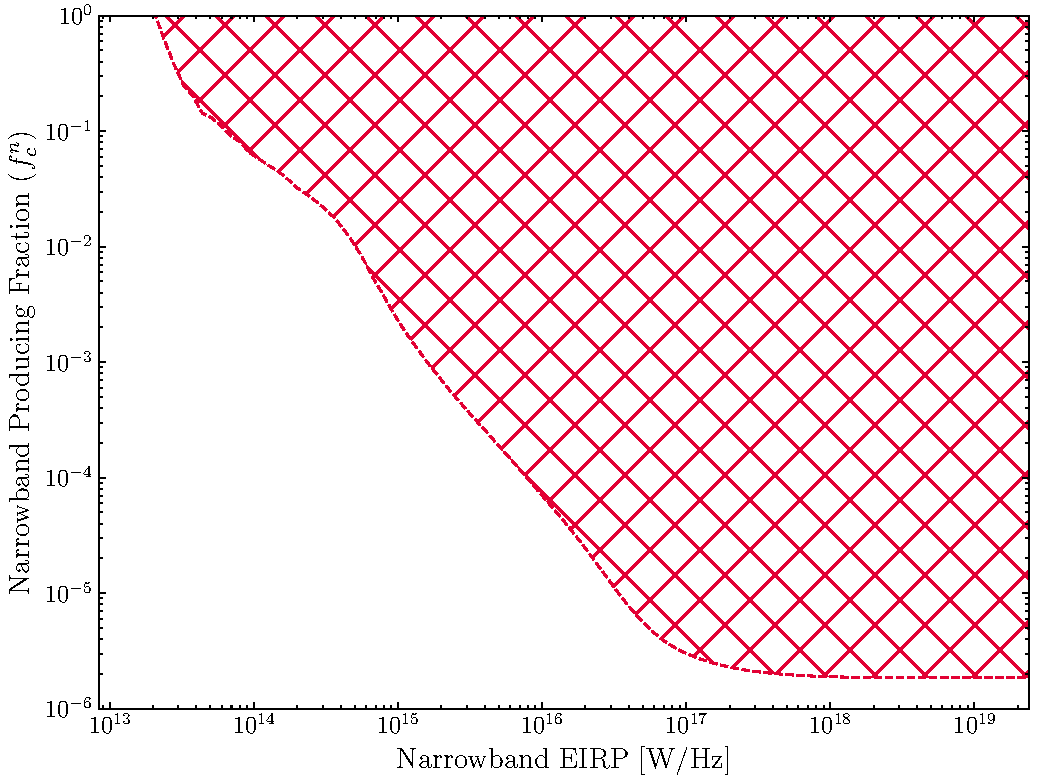
\includegraphics[width = 0.5\textwidth]{figs/narrowband-fraction.pdf}
    \caption{The fraction of stars that produce narrow-band emission ($f^n_c$) against the transmitter power of the total target pool. The hashed region (red) shows the constraints this survey places on a value of $f^n_c$ at 110 - 190 MHz.}
    \label{fig:SETI-constraint}
\end{figure}



\subsection{Search for Extraterrestrial Intelligence}
\subsection{M-dwarf Radio Flares}
% \section{Professional Development}

% Sine the beginning of my PhD I've actively been taking steps as a to develop my skills for a career in research. This takes the form of completing classes, attending conferences and giving presentations on my work to date. \\ 

% As part of my mandated learning credits both took and audited the following modules. 

% \begin{enumerate}
%     \item Overlaps at the Frontiers of
% Astrophysics, Cosmology and Particle Physics \hfill (Winter School)
%     \item C Programming \hfill (Audited) 
%     \item Programming with CUDA \hfill (Audited) 
    
% \end{enumerate}

\section{Summary}

\newpage
\bibliography{frb,pulsar}       % Multiple bib files.

\newpage
\printindex
\end{document}

